\section{Schaltende Regler}

\subsection{Klassifizierung von Regelstrecken oder Modellen}

\begin{itemize}
    \item statisch $\leftrightarrow$ \underline{dynamisch} 
    \begin{itemize}
        \item Drehzahlregelung eines Getriebes?
        \item Stromregelung eines Widerstandes?
    \end{itemize}
    \item akausal $\leftrightarrow$ \underline{kausal}
    \begin{itemize}
        \item Eine Strecke reagiert immer unmittelbar oder verzögert aber nie 'im Voraus' reagieren
        \item Ein Regler kann nicht verfrüht auf eine Störung
    \end{itemize}
    \item \underline{linear} $\leftrightarrow$ nichtlinear
    \item \underline{zeitinvariant} $\leftrightarrow$ zeitvariant
    \item \underline{mit Ausgleich} $\leftrightarrow$ ohne Ausgleich
    \item \underline{konzentrierte Parameter} $\leftrightarrow$ verteilte Parameter
    \begin{itemize}
        \item ODE vs. PDE
    \end{itemize}
    \item \underline{deterministisch} $\leftrightarrow$ stochastisch
    \begin{itemize}
        \item Führungsgrösse: Deterministisch
        \item Störgrösse: Stochastisch
    \end{itemize}
\end{itemize}


\subsection{Stetiger Regler vs. Schaltende Regler}

Ein \textbf{stetiger Regler} kann/soll auf \textbf{kleine Änderungen} der Signale reagieren \\
(z.B. 16 Bit A/D-Wandler) 

\vspace{0.2cm}

Einem \textbf{schaltenden Regler} stehen Signale nur in \textbf{beschränkter Auflösung} zur Verfügung - oft nur 1 Bit. 
Ein zu schnelles Hin- und Herschalten des Reglers wird oft durch eine \textbf{Hysterese} verhindert. 


\subsection{Zweipunktregler (Strecke: Integrator)}{64}

\vspace{-0.2cm}
$$ \boxed{\text{Fehler:} \quad e(t) = r(t) - y(t)} $$
\begin{center}
    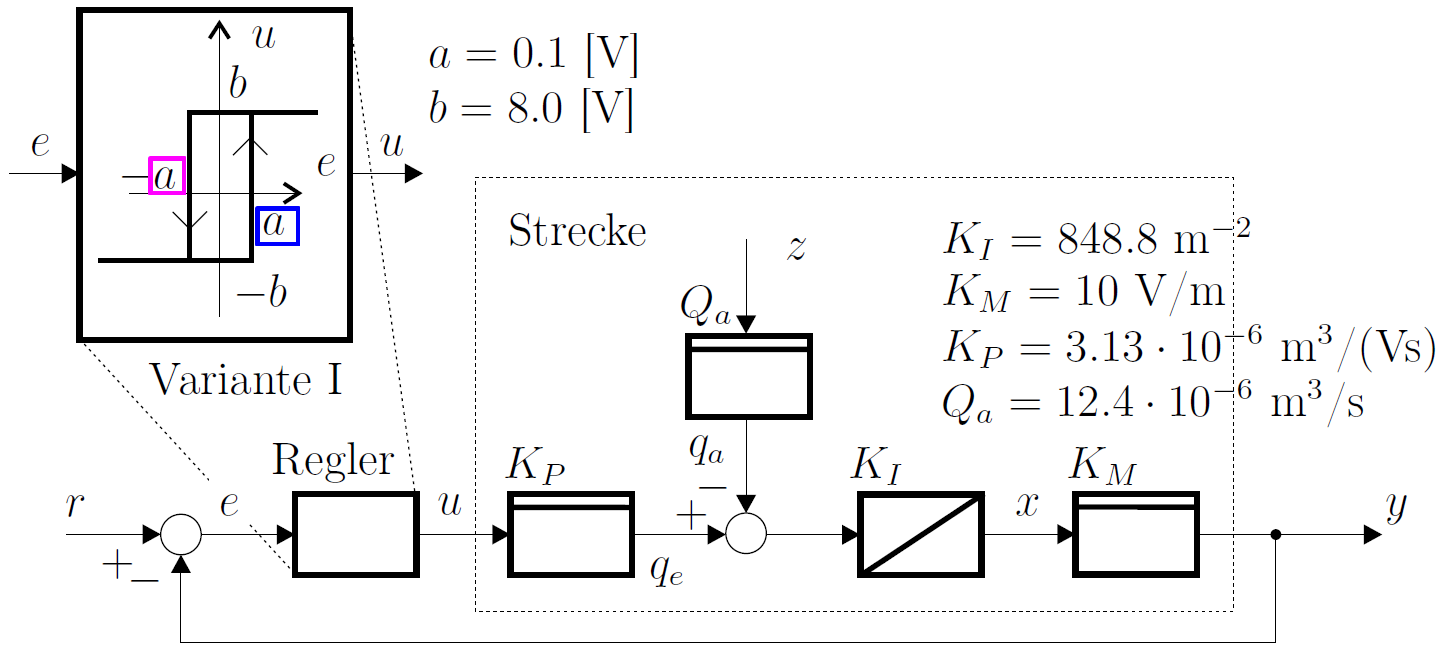
\includegraphics[width=0.85\columnwidth]{images/zweipunkteregler_beispiel.png} 
\end{center}


\subsubsection{Berechnungen am Grenzzyklus}{65-66}

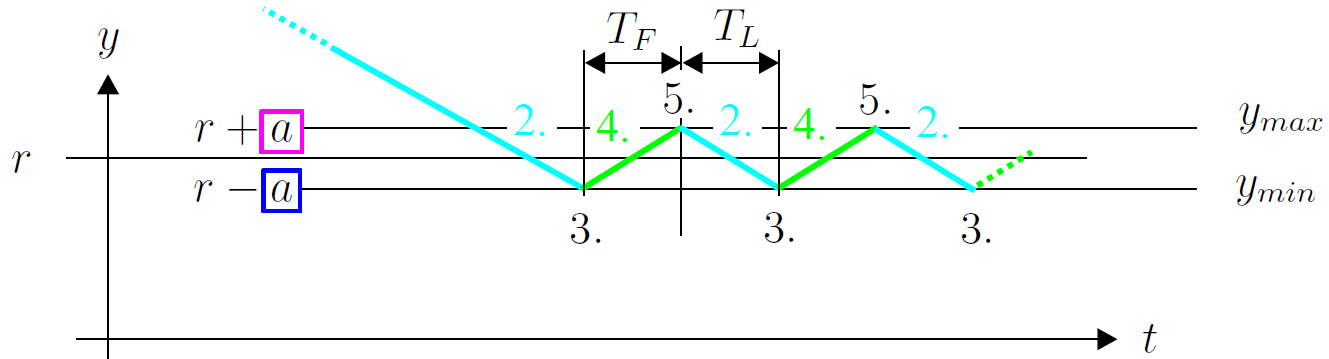
\includegraphics[width=\columnwidth]{images/grenzzyklus.png}

\fbox{\parbox{0.96\columnwidth}{
    \renewcommand{\arraystretch}{1.7}
    \begin{tabular}{ll}
        $y_{\rm max}$   & Maximalwert von $y$ während des Zyklus                                \\
        $y_{\rm min}$   & Minimalwert von $y$ während des Zyklus                                \\
        $\Delta y $     & $\Delta y = y_{\rm max} - y_{\rm min}$ \quad (Schwankungsbereich)     \\
        $y_m$           & $y_m = \frac{y_{\rm max} + y_{\rm min}}{2}$ \quad (Mittelwert)        \\
        $T$ 	        & Periodendauer des Grenzzyklus
    \end{tabular}  
    \renewcommand{\arraystretch}{1}

    $$ T = T_F + T_L = \frac{y_{\rm max} - y_{\rm min}}{K_M \, K_I \, K_P  \,b} + \frac{y_{\rm min} - y_{\rm max}}{- K_M \, K_I \, K_P  \,b} = \frac{4 \, a}{K_M \, K_I \, K_P  \,b} $$
} }
  
  

\subsection[Zweipunktregler (Strecke: PT1 mit Totzeit)]{Zweipunktregler (Strecke: $\text{PT}_1$ mit Totzeit)}{68}

\begin{minipage}[c]{0.65\columnwidth}
    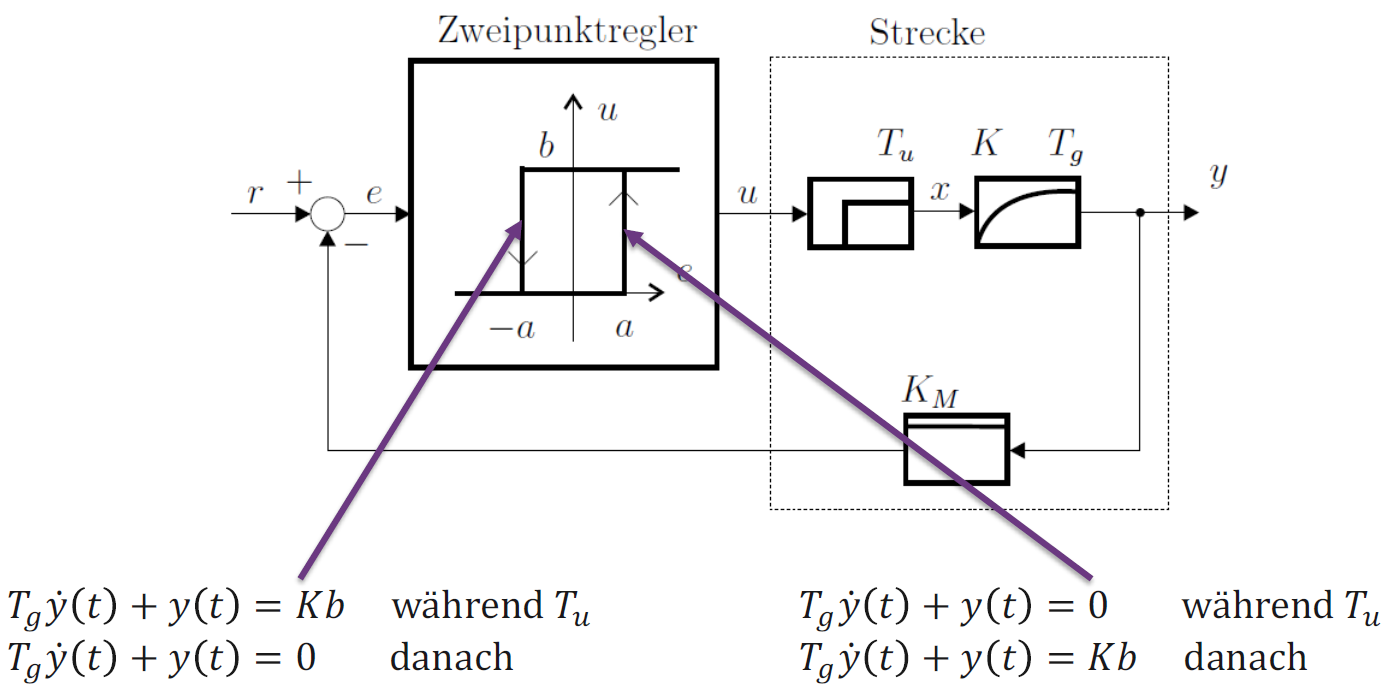
\includegraphics[width=\columnwidth]{images/zweipunkteregler_PT1.png}
\end{minipage}
\hfill
\begin{minipage}[c]{0.33\columnwidth}
    $$ \boxed{e(t) = r(t) - y(t) }$$
\end{minipage}

\begin{center}
    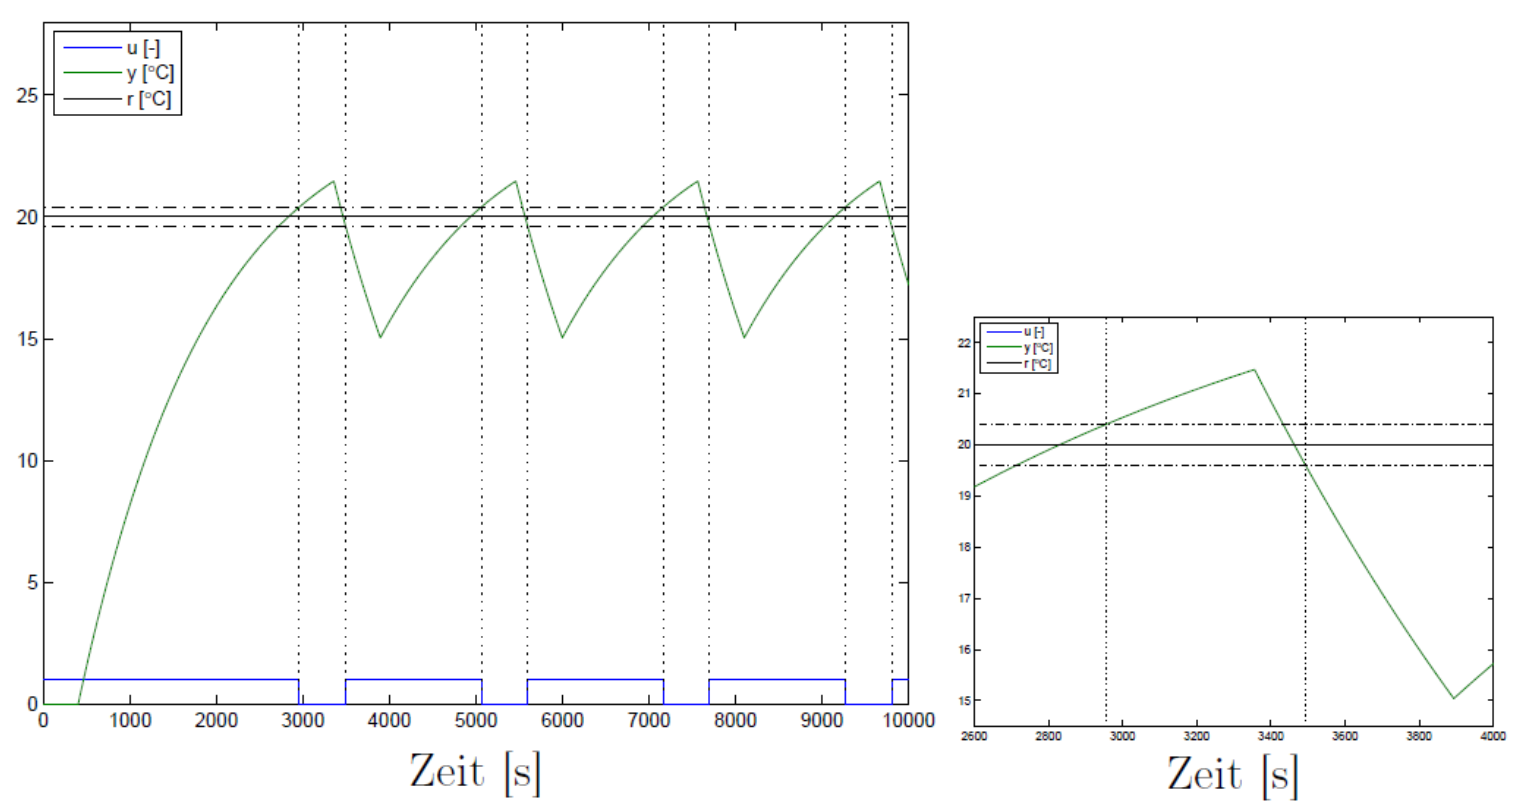
\includegraphics[width=0.9\columnwidth]{images/zweipunkteregler_PT1_simulation.png} 
\end{center}

\begin{enumerate}
    \item $y(t)$ wegen Totzeit nicht in Toleranzband $r \pm a$
    \item $y(t)$ ist im Mittel $y_m$ deutlich unterhalb von $r$
    \item Berechnungen werden viel aufwändiger
    \item Kennwerte ($y_m, \, T, \ ...$) sind von Amplitude abhängig 
\end{enumerate}


\subsubsection{Berechnungen am Grenzzyklus}

\begin{center}
    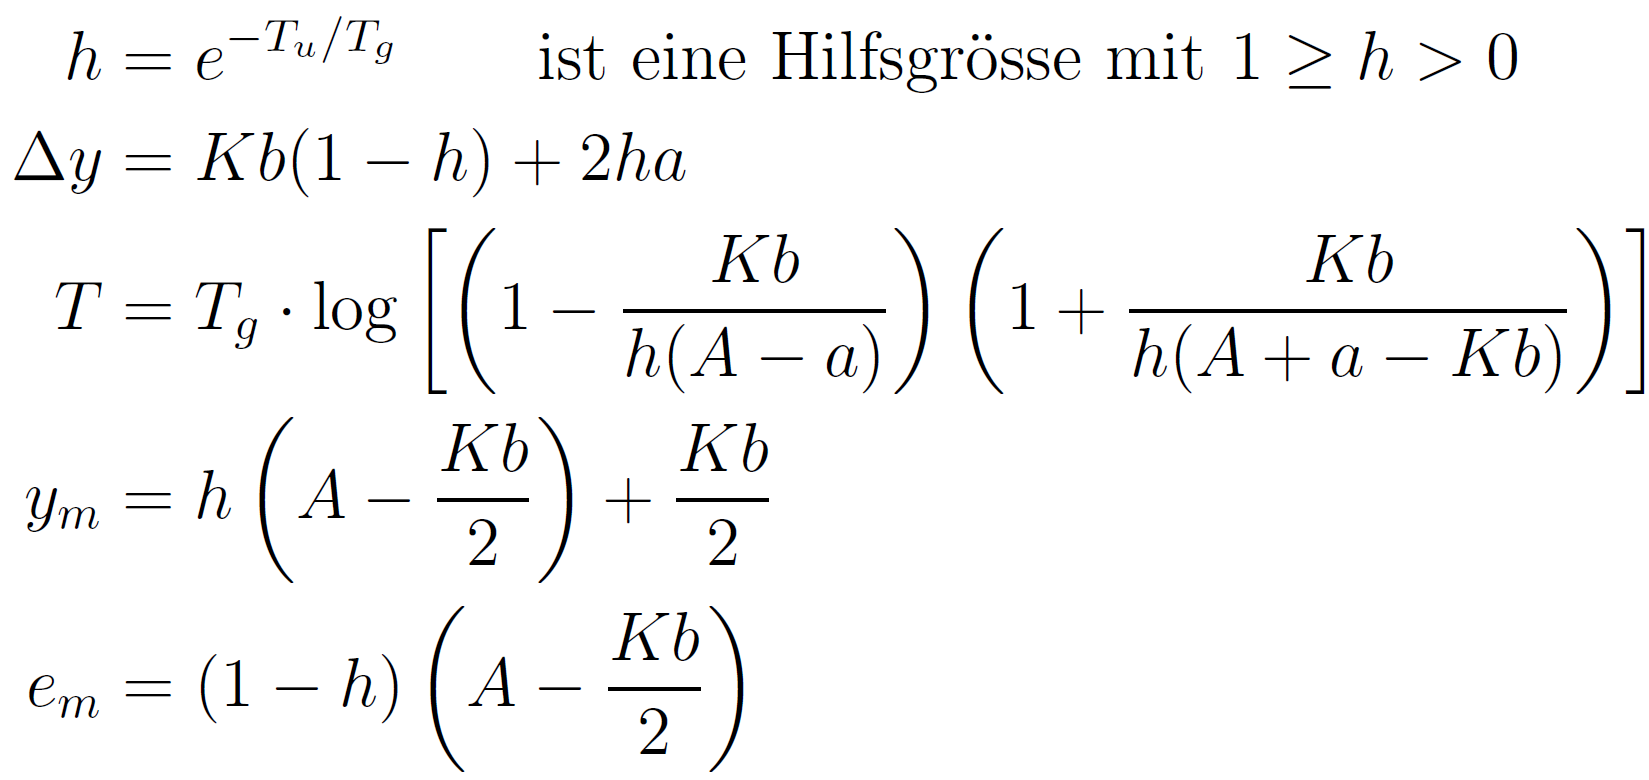
\includegraphics[width=0.7\columnwidth]{images/zweipunkteregler_PT1_berechnungen.png} 
\end{center}


\subsection{Dreipunkteregler / Mehrpunkteregler}{71}

\begin{minipage}[c]{0.3\columnwidth}
    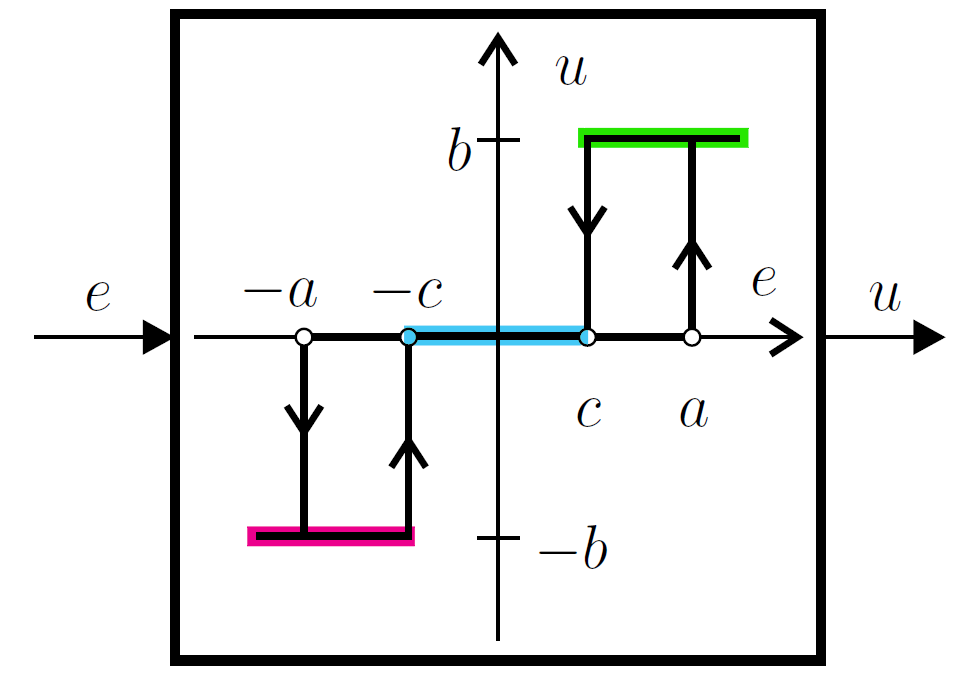
\includegraphics[width=\columnwidth]{images/dreipunkteregler.png}
\end{minipage}
\hfill
\begin{minipage}[c]{0.66\columnwidth}
    \raggedright
    Ein Dreipunkteregler hat drei mögliche Werte für das Stellsignal $u(t)$, z.B. vorwärts, aus und rückwärts. 
    Die Realisierung kann z.B. mit \textbf{zwei Hysteresen} erfolgen, wobei sich \textbf{vier Schaltbedingungen} ergeben. 
\end{minipage}

